\documentclass[11pt,a4paper]{article}

\usepackage{polski}
\usepackage[utf8]{inputenc}
\usepackage{graphicx}
\title{Wstęp do obliczeń ewolucyjnych i neuronowych -- zadanie 1}
\author{Maciej Andrejczuk}
\date{2011-02-24}

\begin{document}
\maketitle

\begin{abstract}
Zadanie przygotowawcze polega na wielokrotnym symulowaniu 'procesu kolekcjonowania kuponów'.
Polega on na losowaniu (ze zwracaniem) kuponów (liczb z przedziału $1..K$) aż do momentu wylosowania każdego kuponu (liczby) co najmniej raz.

\end{abstract}

\newpage

\tableofcontents

\section{Opis algorytmu zastosowanego do rozwiązania problemu}

Program wykonuje $M$ eksperymentów, podczas każdego z nich losuje $N$ liczb.
Po każdym losowaniu sprawdza (w tablicy, w czasie stałym), czy wylosowana liczba już wystąpiła i ją zapamiętuje.
Zbiera też dane niezbędne do obliczenia statystyk: wartości średniej, odchylenia standardowego, minimum i maksimum.

%\newpage
\section{Opis i dyskusja eksperymentów}

Liczba kuponów K została ustalona w treści zadania na $K = 100$.
Parametry N (liczbę zakupów) oraz M (liczbę eksperymentów) ustaliłem ręcznie: $N = 1200$, $M = 50000$.
Wtedy spełnione są warunki postawione w treści zadania:
\begin{itemize}
\item Wartość N powinna być taka, żeby z wykresu można było zorientować się ile (z grubsza) zakupów powinien wykonać zbieracz,
aby osiągnąć cel.
\item Wartość M powinna być dostatecznie duża, aby umożliwić uzyskanie w miarę „regularnego” wykresu średnich (tzn. zapewnić dostatecznie małe odchylenia standardowe).
\end{itemize}

%newpage
\section{Wyniki}

Wykres przedstawia minimalne, maksymalne oraz średnie ilości zebranych
kuponów w zależności od ilości zakupów:

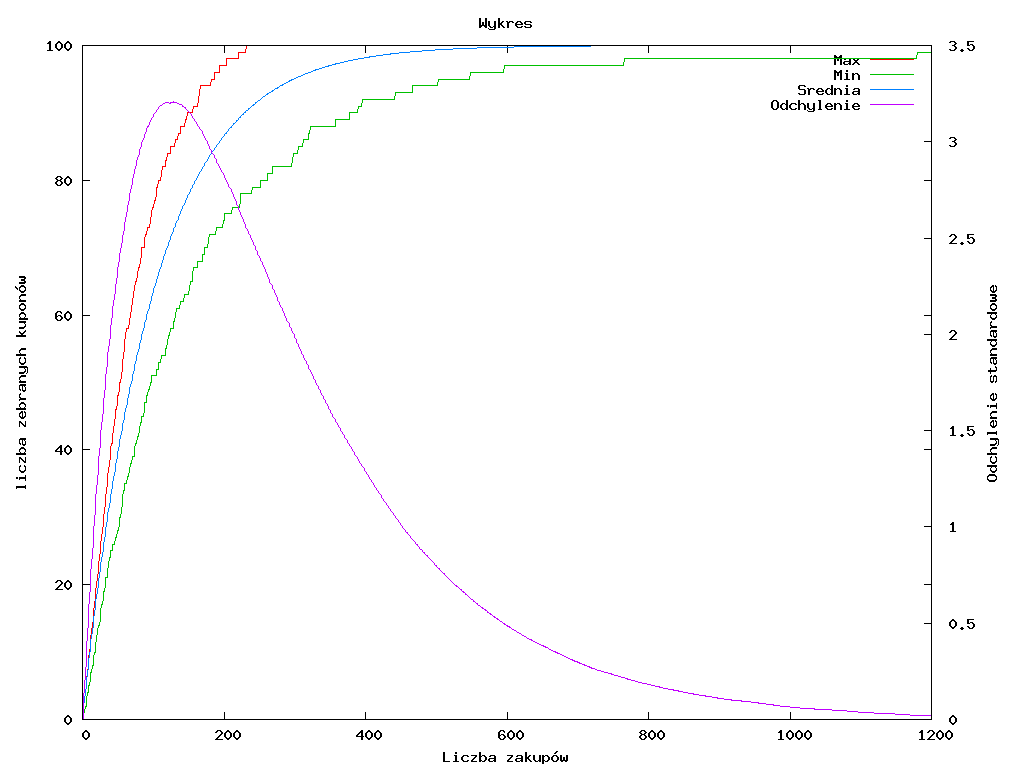
\includegraphics[width=15cm]{wykres.png}

Z wykresu wynika, że należy wykonać ok. $600$ zakupów, aby średnia ilość wylosowanych kuponów zbliżyła się znacząco do $100$ 
(wynosi ona wtedy $99.75692$, czego na wykresie uchwycić już się nie da...).

\end{document}
